% Related works section
In this section, we briefly introduce existing literature on persuasive communication (\S\ref{rel:pers}) and distinguish persuasiveness from two commonly confounded traits, sensationalism (\S\ref{rel:viral}) and memorability (\S\ref{rel:mem}). We provide some background on deep learning models for text generation (\S\ref{rel:nlg}) and expand on two types: autoregressive models (\S\ref{rel:autoreg_models}) and non-autoregressive models (\S\ref{rel:non_autoreg_models}). We then expand on techniques to generate persuasive text, such as textual style transfer (\S\ref{rel:tst}) and controllable natural language generation (\S\ref{rel:control}).

\section{Persuasive Communication}
\label{rel:pers}
Persuasiveness is a highly audience-dependent stylistic objective \citep{duerr-2021}, and there is considerable debate in advertising literature on a precise definition. \citet{iyer2019unsupervised} define persuasion as having one party trying to convince another to elicit some behavior, whether a direct action or simply a change in belief. \citet{hidey-etal-2017-analyzing} analyze the Aristotelian modes of persuasion - ethos, pathos, and logos - finding that the latter two, when used in conjunction, significantly affect the persuasiveness of arguments. \citet{demers_2016} collates various persuasion studies into six interventions to achieve persuasiveness, including speaker confidence, patience, persistence, and the introduction of logical argumentation and flattery. In language expectancy theory, there is an expectation that individuals with low credibility are severely restricted in persuasion techniques as opposed to individuals with high credibility, who have the freedom to select various language strategies \citep{burgoon1993interpersonal}. For instance, an individual with low credibility tends to succeed more with a low-intensity attack strategy when trying to overcome resistance to persuasion.

Many existing works have found that persuasive messaging strongly correlates with certain linguistic features. \citet{cano-basave-he-2016-study} find that persuasive language is characterized by techniques that create urgency, such as the use of emotive lexicons and alliteration. \citet{tan2016} and \citet{li2020} find linguistic patterns, interaction dynamics, and discourse structure are strong identifiers of persuasive arguments. Further, \citet{tan2016} states that persuasive arguments are generally calmer, slightly less happy, and have high lexical diversity. \citet{duerr-2021} presents an extensive list of determinants for four categories of persuasive language: benevolence, linguistic appropriacy, logical argumentation, and trustworthiness. They include features that can be quantitatively measured, such as usage of emotionality, evidence words, downtoners, amplifiers, repetition, and much more. \citet{duerr-2021} also include qualitative determinants such as scarcity and authority, but these are hard to measure and control given a textual dataset. \citet{habernal-gurevych-2016-argument} created a rich suite of lexical linguistic features to predict arguments labeled as convincing by annotators, finding that an SVM trained on these features could outperform a Bi-directional LSTM trained on just the text.

We find a need for more work on the unconstrained generation of persuasive and memorable text~\citep{duerr-2021, van-noort-2020-automatic}. There is some related work on generating persuasive/memorable content in other domains such as image and video \citep{liu2021ai, kyle2020generating}, but they struggle to generalize to text. \citet{lipa-urbina-2021} utilize the SentiGAN \citep{sentigan-wang} framework to generate persuasive messages based on the Cialdini principles \citep{cialdini2009influence}. However, the quality and size of their training data limited their results and constrained generation to a specific set of principles, inhibiting other features of persuasiveness. \citet{chen2022generating} propose a novel multi-aspect multi-source generation model to generate persuasive responses to online reviews. However, their definition of persuasion is severely restricted, lacking generalizability to different tasks and audiences.


Due to the disputed definition of persuasiveness, it is often confounded with other styles, namely sensationalism, and memorability. In the following two subsections, we discuss existing work on generating viral/sensational (\S\ref{rel:viral}) and memorable (\S\ref{rel:mem}) content, along with their differences from persuasion.

\subsection{Viral \& Sensational Content}
\label{rel:viral}
Viral and sensational content are often confounded with persuasion, and it is crucial to make a distinction in the definition. Sensational content aims to diffuse quickly and widely in a community by eliciting actions, such as clicks and shares \citep{guerini2012linguistic}. However, the goal of persuasion, while not wholly distinct, extends beyond sensational content to elicit behaviors such as a change in belief or other actions, such as donating to charity \citep{wang2019persuasion}. \citet{guerini2012linguistic} study how linguistic style and readability of scientific abstracts affect virality. They find features that impact virality across four dimensions - certainty, time-related, self-centered, and sense-related - including a positive correlation with future form verbs and a negative correlation with past tense verbs, more prominent use of self-centered pronouns, and a tendency to describe through sense-related verbs, similitudes, and terms related to social interaction. They also find that while all abstracts have high-difficulty readability scores, highly bookmarked articles tend to have higher (i.e., more complex) readability scores, and highly downloaded articles tend to have smaller readability scores. \citet{xu2019clickbait} look at generating sensational headlines using a novel auto-tuned reinforcement learning loss function. They train a sensationalism scorer to label how sensational online headlines are and use it to train a pointer-generator architecture to generate sensational content. While their work served as a strong influence, their use of direct scoring is not robust to many scenarios, and the scope of generation is heavily limited because of the pointer-generator.

\subsection{Memorable Content}
\label{rel:mem}
Like sensationalism, memorability is often confounded with persuasion, and it is again necessary to make a distinction. There is no conclusive study on whether persuasion and memorability are equivalent or are subsets of one another \citep{goode2007implicit}; however, we can understand the differences through the goals of each. While persuasion attempts to change behaviors or to do something, memorability has the goal of lasting within a target audience's consciousness for an extensive period \citep{danescu-niculescu-mizil-etal-2012-hello}. \citet{danescu-niculescu-mizil-etal-2012-hello} investigate language-based memorability by analyzing a list of memorable movie quotes, finding that the usage of distinctive language, common syntactical structures, fewer third person pronouns, more present tense verbs, and fewer past tense verbs, among other things, are strongly correlated with memorability. Other existing work has studied culturally significant text in the context of long-term memory and found that poetic rhetorical devices (e.g., alliteration) help contribute to the auditory and rhythmic nature of memorable text \citep{rubin1977very, hyman1990memorabeatlia, boers2005finding}.

\section{Deep Learning Models for Text Generation}
\label{rel:nlg}

Deep learning has provided many techniques for text generation, which fall into two categories: autoregressive and non-autoregressive models. In the following two subsections, we define and explore related work in autoregressive (\S\ref{rel:autoreg_models}) and non-autoregressive (\S\ref{rel:non_autoreg_models}) text generation.

\subsection{Autoregressive Models}
\label{rel:autoreg_models}

Autoregressive models are feed-forward models that predict the next word given an existing sequence and, in the text domain, are typically language models (LMs). More formally, at time $t$, given the sequence $x_1, x_2, ... x_{t-1}$, the model outputs $P(x_t | x_1, x_2, \dots x_{t-1})$, the predictive probability distribution for $x_t$. Language models (LM) aim to estimate the probability of a given sequence of words, fundamentally making them a good candidate for autoregressive modeling. 

Recently, LMs have been scaled up from a few million parameters to hundreds of millions of parameters to hundreds of billions of parameters \citep{brown2020language}, using massive corpora of text for training. Examples of these large language models (LLMs) include BERT \citep{devlin-etal-2019-bert}, GPT \citep{radford2018improving, radford2019language, brown2020language}, XLNet \citep{yang2019xlnet}, and RoBERTa \citep{liu2019roberta}. In Chapter \ref{chp:style_infusion}, we utilize GPT-2 for its extensive pretraining and versatility during training for task-specific open-ended generation.

While autoregressive models are very powerful, their sequential nature makes them slow and prone to consistency/repetition errors as the sequence grows longer \citep{bender2021dangers}. Many solutions have been proposed for these issues, such as adding a repetition penalty during decoding \citep{he2021parallel} and long-document attention mechanisms \citep{beltagy2020longformer}, but this remains an open problem for pretrained language models.

\subsection{Non-Autoregressive Models}
\label{rel:non_autoreg_models}

Non-autoregressive models for text generation cover a broad category of models from variational auto-encoders (VAEs) \citep{kingma2013auto} and energy-based models (EBMs) \citep{deng2020residual} to generative adversarial networks (GANs) \citep{goodfellow2020generative} and most recently, diffusion models \citep{ho2020denoising}. 

\begin{figure*}[ht]
  \centering
  \caption{A graphical representation of generative adversarial networks (GANs) (diagram from \citet{cai2020utilizing}) and variational autoencoders (VAEs). Note that in VAEs, we assume the latent space is Gaussian and sample $z$ from $\mathcal{N}(\mu_x, \sigma_x)$ where the encoder, $q_{\phi}(z | x)$ outputs the mean, $\mu_x$, and standard deviation, $\sigma_x$, of the approximate posterior for a sample $x$.}
  \label{fig:vae_gan}
  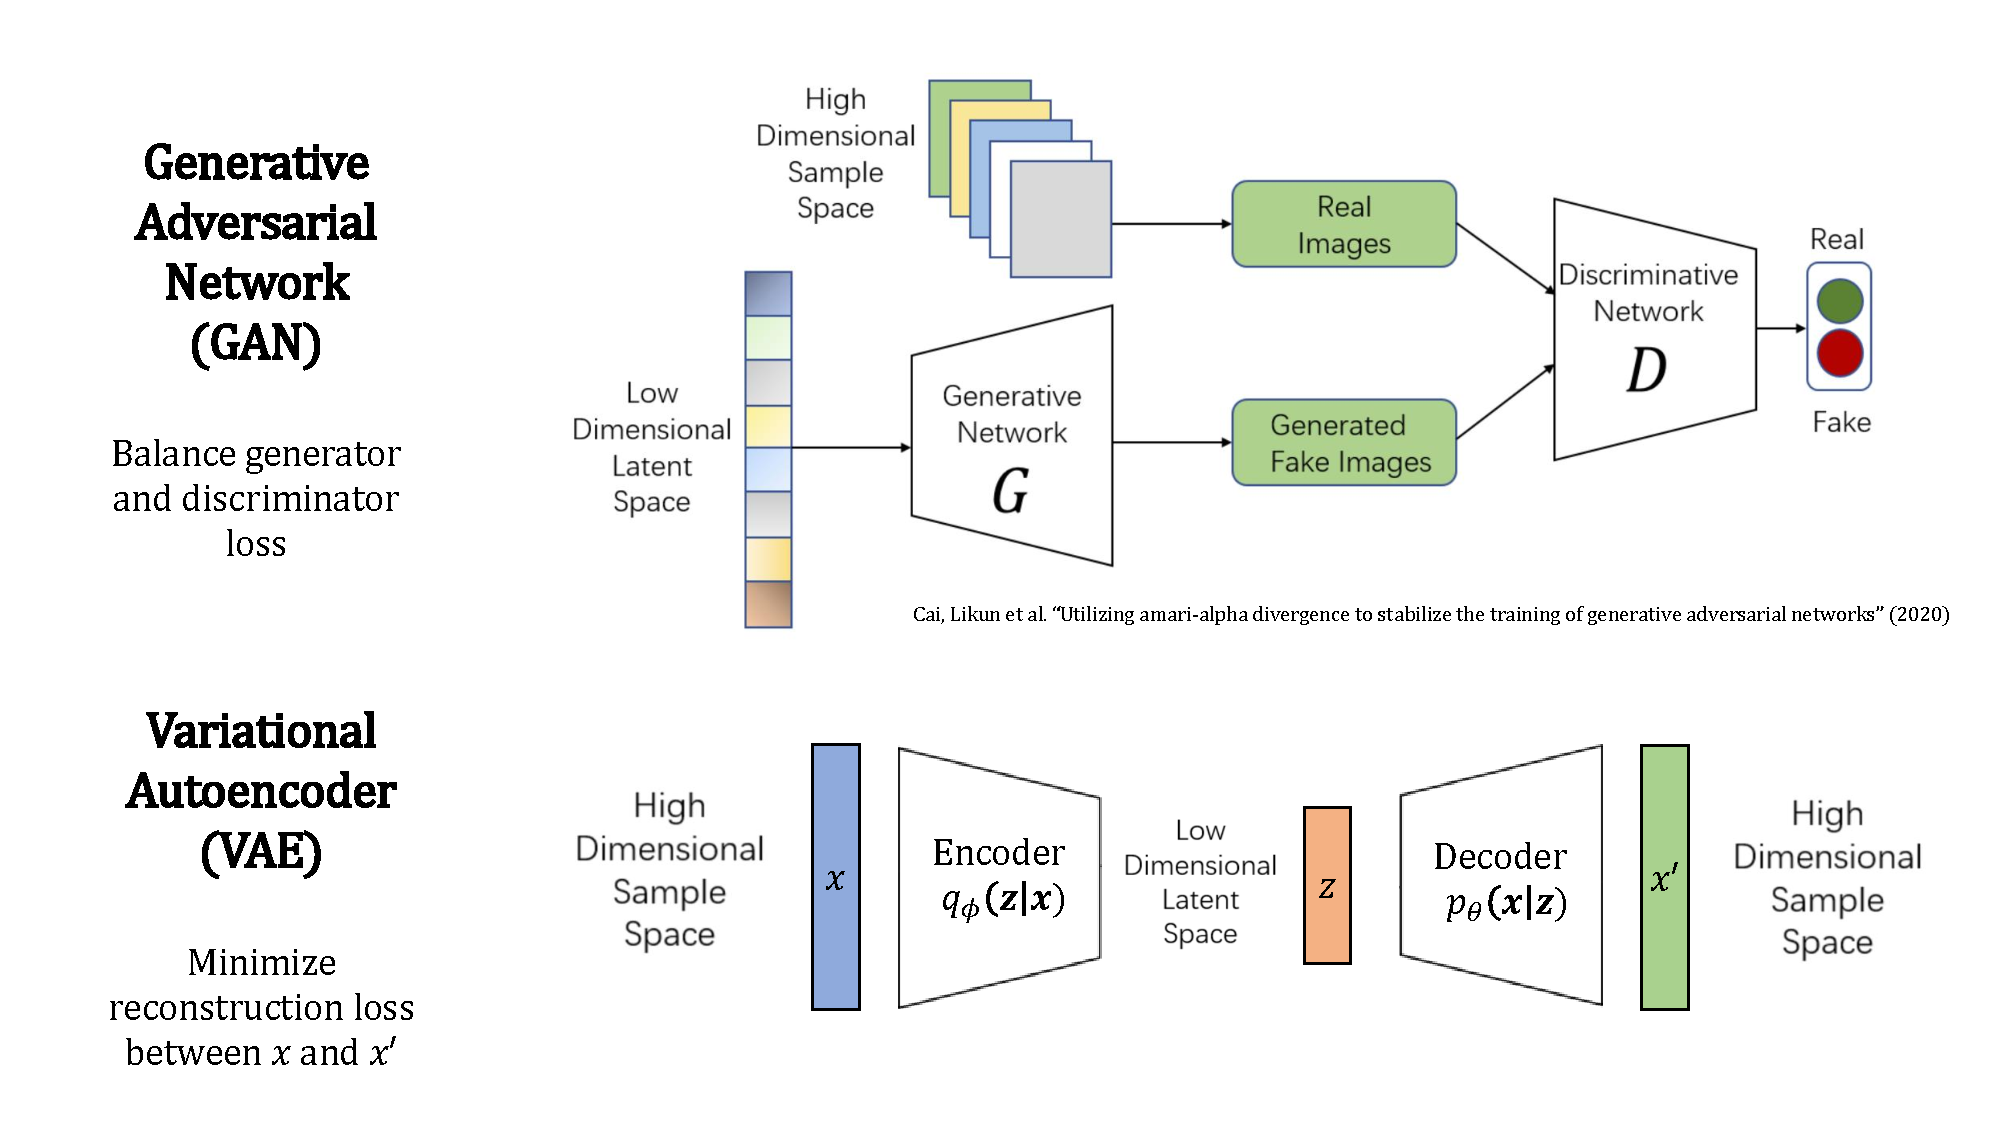
\includegraphics[width=\linewidth]{figs/gan_vae.pdf}
\end{figure*}

Generative Adversarial Networks (GANs) \citep{goodfellow2020generative} estimate generative models through adversarial training with two models: a generator that captures the data distribution and a discriminator which estimates whether a sample came from the generator as opposed to the training data. GANs have been empirically shown to generate higher-quality samples than VAEs \citep{bond2021deep} but require more tuning to synchronize the two models and are prone to problems like vanishing gradients \citep{arjovsky2017towards}, mode collapse, and catastrophic forgetting \citep{thanh2020catastrophic}.

Variational Auto-Encoders (VAEs) \citep{kingma2013auto} are powerful deep generative models that work on unlabeled data and are straightforward to train, as opposed to GANs which require many training tricks for convergence \citep{bond2021deep}. VAEs attempt to map some input $x$ to a latent representation $z$ that can be reconstructed to $x'$, such that the difference between $x$ and $x'$ is minimal. VAEs comprise two jointly learned models: a probabilistic encoder, $q(z|x)$, and a probabilistic decoder, $p(x|z)$.

% \begin{figure*}[ht]
%   \centering
%   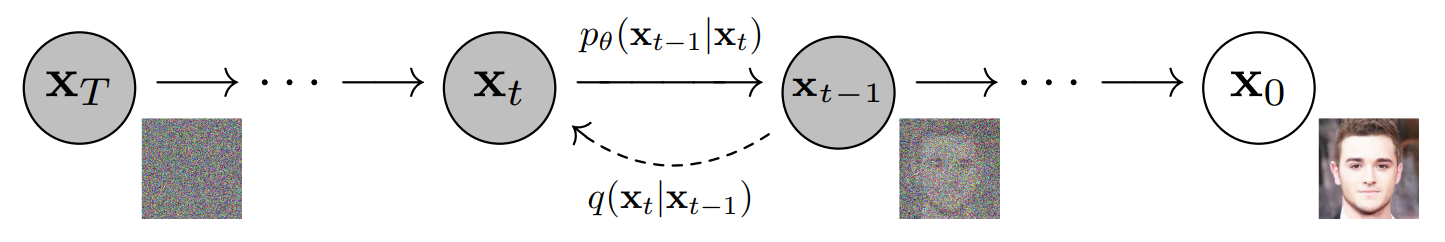
\includegraphics[width=\linewidth]{figs/rel_diffusion.png}
%   \caption{A graphical representation of the forward and reverse diffusion processes in the image domain \citep{ho2020denoising}.}
%   \vspace{0.1in}
%   \label{fig:diffusion}
%   \vspace{-5pt}
% \end{figure*}

% Diffusion probabilistic models (\ie diffusion models) \citep{ho2020denoising} are parameterized Markov chains that learn to reverse an incremental noising process to approximate samples from the target data distribution. Training a diffusion model consists of a forward and backward process. The former incrementally adds Gaussian noise to a data point until at step $T$, the latent representation is approximately Gaussian. The latter learns a parameterization $p(x_{t-1} | x_t)$ to mimic the reverse of the noising function $q(x_t | x_{t-1})$. Diffusion models have been applied in continuous domains to allow for language modeling through diffusion. \citep{li2022diffusion} show that these models are capable of learning complex controls that autoregressive models have failed on. 

\section{Textual Style Transfer}
\label{rel:tst}

Prior work has explored textual style transfer in diverse settings ranging from ``clickbait'' headlines to formalizing text \citep{jin2020hooks, chawla-yang-2020-semi, xu2019clickbait}. While strictly supervised approaches show high fidelity to input samples~\citep{hu2017toward, jhamtani-etal-2017-shakespearizing}, unsupervised and minimally supervised learning are widely applicable since parallel samples are unavailable \citep{shen2017style, yang2018unsupervised}.

Disentanglement, prototype editing, and pseudo-parallel corpus creation are popular approaches for non-parallel data. Prototype editing applies stylistic markers to predefined sentence templates, replacing unwanted parts of the text with text that conforms to a desired attribute \citep{guu2018generating, li-etal-2018-delete}. Disentanglement extracts style independent of the content in a latent space \citep{shen2017style, hu-et-al-controllable}. Pseudo-parallel corpus construction aligns sentences from two mono-style corpora \citep{jin-etal-2019-imat, zhang2018style}. Audience-centric feedback may not conform to the rigid hypotheses of prototype editing and disentanglement. In the case of the former, unconstrained generation allows for freedom in sentence and paragraph-level constructs to define the style \citep{li2020}. For the latter, the separability of content and style is more challenging in specialized domains reliant on domain-specific jargon \citep{woodward2008more} and expressions. Our bootstrapping approach shares some commonalities with pseudo-parallel corpus creation \citep{jin-etal-2019-imat, zhang2018style}, but only utilizes a generic topical corpus to expand the audience-generated ``seed set'' of pairwise judgments. 

Adversarial training has also been used to quantify style \citep{yang-2022-adversarial, John2018}, specifically in disentanglement. \citet{John2018} use auxiliary adversarial and multi-task training objectives to disentangle content from style. For both style and content, they create a multi-task loss to ensure the functionality of the latent representation and an adversarial loss to ensure style does not bleed into content and vice versa. Our approach explicitly decouples the style discrimination and generation tasks for modularity and incremental training purposes, leading to a more robust representation of style.

The evaluation of textual style transfer is generally broken into three parts: fluency, semantic preservation, and strength of the transferred style. Fluency and semantic preservation are well-explored metrics with existing automatic evaluation techniques such as BLEU \citep{Papineni2002bleu}, ROUGE \citep{lin-2004-rouge}, language model perplexity, and BERTScore \citep{zhang2019bertscore}. Most works often use a separately trained stylistic discriminator for automatically evaluating the transferred style strength; however, a robust and reliable classifier requires additional high-quality labeled data, which is problematic in low-resource scenarios. Our approach utilizes the existing pairwise judgments to learn how different linguistic features contribute to the strength of the transferred style.

\section{Controllable Text Generation}
\label{rel:control}

Controllable text generation (CTG) is a fundamental task in natural language generation with a wide variety of applications, such as emotional control in dialogue generation and ensuring that toxic, biased, or discriminatory language is not used in generation. Early literature relied on deep generation models such as variational auto-encoders (VAEs) \citep{guu2018generating, xu2020variational, wang2019topic} and generative adversarial networks (GANs) \citep{scialom2020discriminative} because of the capability of the learned low-dimensional representation to represent linguistic features. \citet{guu2018generating} propose a prototype-then-edit model which generates a sentence by randomly sampling an example from the training set and then applying a randomly sampled edit vector. \citet{scialom2020discriminative} use a GAN-style architecture, training a discriminator to guide the generator toward human-style writing. Recently, \citet{li2022diffusion} utilized diffusion models to denoise a sequence of Gaussian vectors into word vectors while controlling the denoising steps with a gradient-based method, allowing for controllable text generation.

With the recent success of pretrained language models (PLMs), current approaches have generally shifted to a plug-and-play approach to exploit the knowledge from PLMs without significant task-specific retraining. \citet{keskar2019ctrl} attempts to retrain a language model conditioned on control codes ranging from styles and domains (\eg science, politics, horror) to links, questions, and languages. \citet{Dathathri2020Plug} propose using the gradients from simple attribute classifiers (\eg bag of words, single learned layer) during sampling to guide the generation of a PLM. 

\citet{krause2020gedi} guides the generation of a larger PLM using two class-conditional language models, one conditioned on the desired control and one conditioned on the ``anti-control''. Their work resolved the expensive decoding problem from \citet{scialom2020discriminative} and inspired many follow-up works \citep{yang2021fudge, liu-etal-2021-dexperts}. \citet{yang2021fudge} adjusts the output logits of any given PLM with a learned attribute predictor that predicts whether an attribute will be true in the future, as opposed to existing work which judges based on the present. 

Many approaches have also attempted to control generations during decoding. \citet{liu-etal-2021-dexperts} steers the output distribution of a PLM with an ensemble of ``expert'' and ``anti-expert'' LMs by obtaining the outputs of all LMs at timestep $t$ based on prompt $x_{<t}$, obtaining $z_t$ (from the PLM), $z_t^+$ (from the ``expert''), and $z_t^-$ (from the ``anti-expert''). The resulting distribution (\ie product-of-experts ensemble) is:

\begin{equation}
    \tilde{P}(X_t | x_{<t}) = \text{softmax}(z_t + \alpha (z_t^+ - z_t^-))
\end{equation}

where $\alpha$ is a hyperparameter that controls the amount of change to $z_t$. \citet{kumar2021controlled} formulates decoding as an optimization problem with multiple differentiable constraints: a primary negative log-likelihood constraint (for fluency) and multiple secondary constraints for desired attributes.

To summarize, existing approaches only empirically evaluate three types of control conditions: semantic (\eg emotion, topics), structural (\eg syntax tree, parts-of-speech), and lexical controls (\eg keyword/phrase inclusion) \citep{Zhang2022ASO}. Furthermore, while some studies claim to support multiple controls during text generation, there has been little evidence for any such technique. Our work addresses the former by exhibiting control over speed \citep{toubia-2021}, a linguistic feature that does not cleanly fall into the three control conditions. We leave it to future work to text and explore methods to condition text on multiple controls effectively.

In the next chapter, we introduce the task of \textit{style infusion} and propose a novel approach to infuse audience-centric styles into pretrained language generation models.




